\documentclass[]{llncs}
\usepackage{tikz}

\author{Valentin Mayer-Eichberger}

\institute{IVU Traffice Technologies\\
Bundesallee 88, 12000 Berlin\\
\email{vme@ivu.de}}

\title{Two ASP Encodings of  Spinpossible}

\newcommand{\spintable}[9]{
\node [matrix,ampersand replacement=\&,nodes={fill=blue!20,minimum size=5mm}] (node#1)
    {
    \node {#1}; \& \node{#2}; \& \node {#3}; \\
    \node {#4}; \& \node{#5}; \& \node {#6}; \\
    \node {#7}; \& \node{#8}; \& \node {#9}; \\
    };
}


\begin{document}
\maketitle

\section{ASP translation}

\subsection{First encoding}

\subsection{Second encoding}

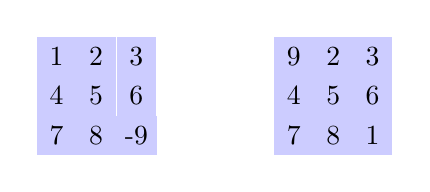
\begin{tikzpicture}
\spintable{1}{2}{3}{4}{5}{6}{7}{8}{-9}
\begin{scope}[xshift=3cm]
\spintable{9}{2}{3}{4}{5}{6}{7}{8}{1}
\end{scope}
\end{tikzpicture}

\paragraph{Replacing numbers by vectors}

\paragraph{Splitting moves/states}

\paragraph{Order on state}

\subsection{Detailed encoding}
\paragraph{States}
\paragraph{Spins}
\paragraph{State Updates}
\paragraph{Initial and final state}
\paragraph{Symmetry breaking}

\end{document}
